\begin{table*}[!tb]
\caption{Five-dataset comparison. Bold/underline mark best/second distinct values among comparable local measurements only; ties share emphasis. Daggered SNS/TW values are published context and excluded from ranking. Curves use fixed default orientations.}
\label{tab:quantitative-final}
\footnotesize
\setlength{\tabcolsep}{1.5pt}
\renewcommand{\arraystretch}{0.85}
\begin{tabular*}{\textwidth}{@{\extracolsep{\fill}}l*{12}{c}lccc@{}}
\toprule
\multirow{2}{*}{Dataset} & \multicolumn{3}{c}{Hilbert} & \multicolumn{3}{c}{Morton} & \multicolumn{3}{c}{TMTM} & \multicolumn{3}{c}{ST-MTM} & \multicolumn{4}{c}{AnchorMTM (ours)} \\
\cmidrule(lr){2-4}\cmidrule(lr){5-7}\cmidrule(lr){8-10}\cmidrule(lr){11-13}\cmidrule(lr){14-17}
 & SNS$\downarrow$ & TW$\uparrow$ & NPE$\downarrow$ & SNS$\downarrow$ & TW$\uparrow$ & NPE$\downarrow$ & SNS$\downarrow$ & TW$\uparrow$ & NPE$\downarrow$ & SNS$\downarrow$ & TW$\uparrow$ & NPE$\downarrow$ & Mode & SNS$\downarrow$ & TW$\uparrow$ & NPE$\downarrow$ \\
\midrule
\multirow{2}{*}{Gaussian} & \multirow{2}{*}{$0.1117$} & \multirow{2}{*}{$0.6719$} & \multirow{2}{*}{$0.7557$} & \multirow{2}{*}{$\underline{0.0393}$} & \multirow{2}{*}{$\underline{0.8333}$} & \multirow{2}{*}{$0.7359$} & \multirow{2}{*}{$0.25^{\dagger}$} & \multirow{2}{*}{$0.77^{\dagger}$} & \multirow{2}{*}{$\underline{0.1118}$} & \multirow{2}{*}{$0.06^{\dagger}$} & \multirow{2}{*}{$1.00^{\dagger}$} & \multirow{2}{*}{$0.1154$} & Exact & $\mathbf{0.0353}$ & $\mathbf{0.9323}$ & $\mathbf{0.0089}$ \\
 &  &  &  &  &  &  &  &  &  &  &  &  & Balanced & $\mathbf{0.0353}$ & $\mathbf{0.9323}$ & $\mathbf{0.0089}$ \\
\multirow{2}{*}{Ring} & \multirow{2}{*}{$\mathbf{0.1252}$} & \multirow{2}{*}{$\mathbf{0.9048}$} & \multirow{2}{*}{$0.5941$} & \multirow{2}{*}{$0.1489$} & \multirow{2}{*}{$0.7619$} & \multirow{2}{*}{$0.6033$} & \multirow{2}{*}{$0.28^{\dagger}$} & \multirow{2}{*}{$0.68^{\dagger}$} & \multirow{2}{*}{$0.1756$} & \multirow{2}{*}{$0.21^{\dagger}$} & \multirow{2}{*}{$0.88^{\dagger}$} & \multirow{2}{*}{$0.2463$} & Exact & $0.1485$ & $\underline{0.8571}$ & $\underline{0.0471}$ \\
 &  &  &  &  &  &  &  &  &  &  &  &  & Balanced & $\underline{0.1334}$ & $\underline{0.8571}$ & $\mathbf{0.0395}$ \\
\multirow{2}{*}{Wildfires} & \multirow{2}{*}{$0.1883$} & \multirow{2}{*}{$0.8303$} & \multirow{2}{*}{$0.3641$} & \multirow{2}{*}{$0.1304$} & \multirow{2}{*}{$0.8758$} & \multirow{2}{*}{$0.1560$} & \multirow{2}{*}{$0.44^{\dagger}$} & \multirow{2}{*}{$0.88^{\dagger}$} & \multirow{2}{*}{$0.2280$} & \multirow{2}{*}{$0.24^{\dagger}$} & \multirow{2}{*}{$0.91^{\dagger}$} & \multirow{2}{*}{$0.3180$} & Exact & $\mathbf{0.0426}$ & $\mathbf{0.9136}$ & $\underline{0.0131}$ \\
 &  &  &  &  &  &  &  &  &  &  &  &  & Balanced & $\underline{0.0447}$ & $\underline{0.8989}$ & $\mathbf{0.0116}$ \\
\multirow{2}{*}{Storms} & \multirow{2}{*}{$0.1290$} & \multirow{2}{*}{$0.7403$} & \multirow{2}{*}{$0.3705$} & \multirow{2}{*}{$0.1180$} & \multirow{2}{*}{$0.7251$} & \multirow{2}{*}{$0.3468$} & \multirow{2}{*}{$0.34^{\dagger}$} & \multirow{2}{*}{$0.71^{\dagger}$} & \multirow{2}{*}{$0.5753$} & \multirow{2}{*}{$0.21^{\dagger}$} & \multirow{2}{*}{$0.94^{\dagger}$} & \multirow{2}{*}{$0.4579$} & Exact & $\underline{0.0790}$ & $\underline{0.8463}$ & $\underline{0.0399}$ \\
 &  &  &  &  &  &  &  &  &  &  &  &  & Balanced & $\mathbf{0.0743}$ & $\mathbf{0.8766}$ & $\mathbf{0.0140}$ \\
\multirow{2}{*}{PM2.5} & \multirow{2}{*}{$0.2386$} & \multirow{2}{*}{$\mathbf{0.8887}$} & \multirow{2}{*}{$0.8090$} & \multirow{2}{*}{$\underline{0.1760}$} & \multirow{2}{*}{$\underline{0.8277}$} & \multirow{2}{*}{$0.8823$} & \multirow{2}{*}{$0.3018$} & \multirow{2}{*}{$0.7781$} & \multirow{2}{*}{$0.5241$} & \multirow{2}{*}{$0.1897$} & \multirow{2}{*}{$0.8224$} & \multirow{2}{*}{$0.5577$} & Exact & $0.1964$ & $0.7884$ & $\underline{0.1390}$ \\
 &  &  &  &  &  &  &  &  &  &  &  &  & Balanced & $\mathbf{0.1636}$ & $0.7657$ & $\mathbf{0.0468}$ \\
\bottomrule
\end{tabular*}
\vspace{2pt}
\begin{minipage}{\textwidth}\footnotesize For the original four inputs, TMTM/ST-MTM Temporal SNS/TW ($\dagger$) are published values; other entries are local measurements. Author inputs and coverage are unconfirmed. Local TW coverage (Gaussian/Ring/Wildfires/Storms) is 64/64, 1/40, 4/32, 11/744; ineligible frames are omitted. Published TW has two-decimal precision. Mode applies only to AnchorMTM. PM2.5 uses 744 shared-input local frames (TW $k=1$, full coverage); its Balanced mode uses the fixed exploratory 5\% case budget, without validation-set budget selection. ST-MTM uses the Storms preset with start frame 0; PM2.5 baseline metrics are all recomputed.\end{minipage}

\end{table*}
\begin{figure*}[!tb]
\paperfigure[.94\textwidth]{figures/volume_gallery.pdf}{fig:volume-gallery}{Recomputed feature positions on Tangaroa and Cylinder using the default-weight volume configuration. Grey reference points and signed-displacement colors connect feature positions to $q$. Each panel reports the feature-pooled mean absolute displacement and NPE (mean per-frame maximum); positive budgets also report maximum attained merge error. Baseline reflection minimizes pooled reference displacement. These runs use the fixed configurations described in the protocol, distinct from the selected geometry-oriented table settings.}
\end{figure*}


\section{Experiments}\label{sec:experiments}
The evidence follows the argument developed above: validate the positional restrictions, measure absolute spatial positioning, then examine how a merge allowance changes displacement. We first establish the data and comparison protocol, use controlled and real trees to test the bounds, and connect the quantitative results to complete temporal maps and their source fields.

\subsection{Experimental Setup}
Five planar inputs are Gaussian (64 frames), Ring (40), Wildfires (32), Storms (744) and hourly PM2.5 (744). The first four use per-frame persistence fractions $(0.001,0.001,0.15,0.105)$ following the ST-MTM benchmark~\cite{STMTM:2026}. They are local reconstructions: three Gaussian peaks, the archived Ring generator, aggregated wildfire radiative power and ERA5 pressure anomalies. PM2.5 interpolates the January 2017 CAQRA hourly fields to a $160\times144$ grid, with 5\% per-frame persistence. Raster lengths are 4096, except Ring's original 196 positions.

The volumes are Cylinder (102 cropped $135\times64\times48$ $Q$-criterion fields, 2\% per-frame persistence)~\cite{Camarri:2005:Cylinder,Weinkauf:SquareCylinder} and Tangaroa (201 $300\times180\times120$ speed fields, range $[0,2]$, absolute persistence 0.2)~\cite{Popinet:2004:Tangaroa}. Within each comparison, methods share fields, retained labels and support geometry.

SNS measures scale-normalized support-distance stress~\cite{Smelser:2025:Scale}; TW measures neighborhood preservation~\cite{Venna:2001:NP}. Absolute positioning uses
\begin{equation}\label{eq:experimental-npe}
\mathrm{NPE}=\frac1T\sum_t\frac{\max_i|x_i^t-q_i^t|}{L}.
\end{equation}
For the original four planar inputs, published TMTM/ST-MTM SNS/TW provide context (daggers in Table~\ref{tab:quantitative-final}); NPE is measured locally. Local TW coverage is 64/64, 1/40, 4/32 and 11/744 for $k=(1,3,5,3)$. PM2.5 and volume scores are all local, with $k=1$ and full coverage. For PM2.5, the first frame with nonconstant anchors and references determines one sequence-wide reflection from the sign of their covariance: TMTM is reflected and ST-MTM is not. Hilbert/Morton use fixed orientations and full-grid ranks. Thus NPE compares a common reference, while SNS/TW evaluate complementary spatial relationships.

Exact uses zero allowance. On the four benchmark inputs, Balanced selects a positive budget from 1--10\% on the first chronological quarter by minimizing the equal-weight normalized NPE/SNS score, with smaller budgets breaking near ties; the resulting budgets are 1, 1, 5 and 10\%. PM2.5 retains its fixed 5\% mode. Sequence-level references and full-sequence reporting include these selection frames. Volume tables use fixed $+x$ references and selected geometry-oriented configurations; their complete parameters are in the supplement. The volume position/distribution figures use a second, common default-weight configuration, with motion-derived direction for Tangaroa and $x$ for Cylinder.

\begin{figure*}[!t]
\paperfigure[.90\textwidth]{figures/budget_distribution_complete.pdf}{fig:budget-distribution}{Recomputed per-frame budget response. Upper row: worst displacement, with quartiles, 5th--95th percentile whiskers, outliers and mean diamonds (square-root scale). Lower row: measured merge error and budget guides. Ring, Storms and PM2.5 use budgets 0, 1, 2, 5, 10 and 20\%; the two default-weight volumes use 0, 2, 5, 10 and 20\%. Orange marks the selected planar modes. Every plotted frame passes its continuous and raster budget checks.}
\end{figure*}
\subsection{Validation of Position Bounds}\label{sec:bounds-eval}

\begin{figure}[!tb]
\centering
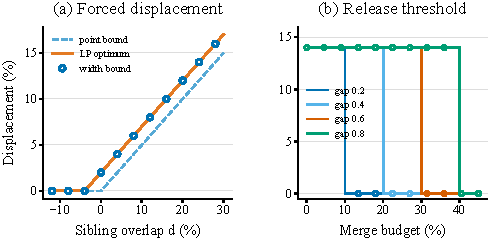
\includegraphics[width=\columnwidth]{figures/anchor_controlled_bounds.pdf}
\caption{Independent four-leaf validation. (a) The width-aware bound and order search coincide with exhaustive minimax LPs over 24 orders. (b) For four parent gaps, the displacement disappears when twice the merge allowance reaches that gap. Circles mark the recomputed bounds.}
\label{fig:controlled}
\end{figure}
To isolate the constraints in RQ1--RQ3, two sibling pairs merge below a root at 1, with leaf values 0 and targets $(0.2,0.5,0.5-d,0.8-d)$. Across 43 overlaps $d\in[-0.12,0.30]$, independent minimax LPs evaluate every leaf permutation. With width 0.06, gap 0.01 and $\rho=0.5$, the exhaustive optimum, width certificate and selected order coincide at $\tau=\max(0,(d+0.04)/2)$ (Fig.~\ref{fig:controlled}a). At $d=0.24$, the point cost is 12\% and the interval cost 14\%.

For parent gaps $h\in\{0.2,0.4,0.6,0.8\}$ and 91 budgets each, all 364 recomputed tests recover the release threshold $2\varepsilon=h$ (Fig.~\ref{fig:controlled}b). These tests connect the three bounds: interleaving causes the point obstruction, widths add packing, and scalar merge gaps determine the price of releasing a block.

\paragraph{Current data sequences.}
The same calculation applies to every frame of our five planar inputs. Table~\ref{tab:real-bounds} recomputes their bounds from the simplified source trees, extremum targets and fixed widths. The selected Exact order attains the width-aware bound on 1,335 of 1,624 frames. On those frames the certificate and an admissible solution coincide, establishing the optimum over all exact-topology orders. Gaussian and Ring attain it on every frame; Wildfires misses it on one and Storms on 15. PM2.5 attains it on 471 of 744 frames and leaves a larger residual gap: mean normalized $\tau$ is 13.11\%, versus a mean bound of 12.88\%. This is the interval-order cost before the capped placement objective chooses the final anchors.

The baseline columns of Table~\ref{tab:real-bounds} distinguish forced displacement from the additional point-order error introduced by each recorded layout. For each frame we sort its recorded anchors and evaluate NROE against the same $q$. The displayed share is $1-\sum_t\nu_t^*/\sum_t\nroe(\pi_t)$, so midpoint ordering removes that share without changing the tree in the point model. On Storms the excess is 91.0\% for TMTM and 83.0\% for ST-MTM; on PM2.5 it is 56.4\% and 59.7\%. The width certificate then identifies the packing cost that remains after order improvement. Together these measurements turn the distinction between forced and chosen displacement into a per-sequence diagnostic.
\begin{table}[!tb]
\centering\caption{Current planar sequences: Exact orders attaining the width-aware lower bound, and the share of local baseline point-order error above the exact point bound. Orientations match the primary measurements.}\label{tab:real-bounds}
\footnotesize\setlength{\tabcolsep}{3pt}
\begin{tabular}{@{}lrrcc@{}}\toprule
Dataset & Frames & Width hits & TMTM excess & ST-MTM excess\\\midrule
Gaussian & 64 & 64 & 100.0\% & 100.0\% \\
Ring & 40 & 40 & 64.5\% & 25.7\% \\
Wildfires & 32 & 31 & 92.5\% & 98.1\% \\
Storms & 744 & 729 & 91.0\% & 83.0\% \\
PM2.5 & 744 & 471 & 56.4\% & 59.7\% \\
\bottomrule\end{tabular}\end{table}

\begin{figure*}[!tb]
\paperfigure{figures/anchor_storms_budget_maps.pdf}{fig:storms-budget-profiles}{Storms event window, frames 355--460, at five AnchorMTM budgets and with local TMTM/ST-MTM maps on the same case-study fields and trees. Common crops and the $[-35,35]$ hPa scale connect the map trajectories to the reference feature.}
\end{figure*}
\subsection{Absolute Spatial Positioning}\label{sec:reference-results}

With the structural cost established, we evaluate the final anchors against the fixed reference. Balanced has lower NPE than the fixed curves and both local merge-tree adapters on all five planar inputs (Table~\ref{tab:quantitative-final}). Against curves, it also improves SNS and TW on Gaussian, Wildfires and Storms. Ring favors Hilbert's SNS/TW (0.1252/0.9048 versus 0.1334/0.8571), and PM2.5 favors Hilbert's TW (0.8887 versus 0.7657). The anchored axis improves location reading while retaining a different balance of local geometry.

\begin{table}[!tb]
\centering
\caption{Volumetric comparison with a fixed $x$ reference. Bold/underline mark best/second distinct values per dataset; ties share emphasis.}
\label{tab:volume-comparison}
\footnotesize
\setlength{\tabcolsep}{1.2pt}
\renewcommand{\arraystretch}{0.9}
\begin{tabular*}{\columnwidth}{@{\extracolsep{\fill}}lccc lccc@{}}
\toprule
\multirow{2}{*}{Dataset} & \multicolumn{3}{c}{TMTM} & \multicolumn{4}{c}{AnchorMTM (ours)} \\
\cmidrule(lr){2-4}\cmidrule(lr){5-8}
 & SNS$\downarrow$ & TW$\uparrow$ & NPE$\downarrow$ & Mode & SNS$\downarrow$ & TW$\uparrow$ & NPE$\downarrow$ \\
\midrule
\multirow{2}{*}{Cylinder} & \multirow{2}{*}{$0.2956$} & \multirow{2}{*}{$\underline{0.8017}$} & \multirow{2}{*}{$0.4769$} & Exact & $\underline{0.1226}$ & $0.8010$ & $\underline{0.1773}$ \\
 &  &  &  & Balanced & $\mathbf{0.0329}$ & $\mathbf{0.9117}$ & $\mathbf{0.0458}$ \\
\multirow{2}{*}{Tangaroa} & \multirow{2}{*}{$0.5255$} & \multirow{2}{*}{$0.6701$} & \multirow{2}{*}{$0.3866$} & Exact & $\underline{0.1204}$ & $\underline{0.8213}$ & $\underline{0.1285}$ \\
 &  &  &  & Balanced & $\mathbf{0.1124}$ & $\mathbf{0.8408}$ & $\mathbf{0.0653}$ \\
\bottomrule
\end{tabular*}
\vspace{2pt}
\begin{minipage}{\columnwidth}\footnotesize All values are local measurements, including adapted TMTM. TW uses $k=1$, with coverage 102/102 and 201/201. Mode applies only to AnchorMTM. Configurations are frozen exploratory results, not a blind test; settings appear in Table~\ref{tab:volume-parameters}.\end{minipage}
\end{table}

In the selected fixed-$x$ configurations, Balanced lowers SNS and NPE and raises TW relative to TMTM on both volumes (Table~\ref{tab:volume-comparison}). Cylinder NPE falls from 47.69\% to 4.58\%; Tangaroa falls from 38.66\% to 6.53\%. The selected Tangaroa configuration has zero reference weight and a 33.33\% allowance, so the mechanism is primarily geometry fitting within the prescribed reference cap.

Figure~\ref{fig:volume-gallery} reveals the spatial patterns behind reference error. Its default Exact configuration has NPE 11.18\% on Tangaroa and 9.18\% on Cylinder, versus TMTM's 30.63\% and 47.69\%. A 5\% budget brings Cylinder to 1.19\%, while Tangaroa reaches 8.91\% and needs 20\% to reach 1.88\%. The grey reference columns show the trajectories against which these displacements are measured.

\begin{figure*}[!tb]
\paperfigure{figures/anchor_cylinder_centered_blue.pdf}{fig:cylinder-centered}{Cylinder: a central-tree guidance variant and five source $Q$ isosurfaces, using a common camera and blue scalar scale. Stages I--V identify early, transition, shedding, transition and late configurations. Its ordinate expresses the guided layout position.}
\end{figure*}
\subsection{Position--Topology Trade-off}\label{sec:relaxation-results}
We next hold the prepared sequence and layout settings fixed and vary the merge allowance. The primary Exact planar runs have zero fixed-leaf merge error. Balanced attains maximum normalized errors 0, 0.982\%, 4.421\% and 9.985\% on Gaussian, Ring, Wildfires and Storms, within their declared budgets. Relative to Exact, NPE decreases by 16.2\%, 11.6\% and 64.9\% on the latter three inputs; Gaussian remains unchanged. Wildfires SNS rises from 0.0426 to 0.0447, showing that improved anchoring can change relative geometry in the other direction.

Figure~\ref{fig:budget-distribution} localizes this improvement. On Storms, a 10\% allowance changes the median displacement from 1.10\% to 0.84\%, but lowers the 90th percentile from 10.7\% to 2.5\%; 482 of 744 frames retain zero merge error. The budget therefore acts chiefly on a difficult tail: its main benefit is concentrated in frames with larger reference conflicts. In the default volumes, 200 of 201 Tangaroa frames and 98 of 102 Cylinder frames use a positive allowance, shifting most of the distribution.

The completed PM2.5 sweep uses the same input, tracks, reference, widths and weights at all six budgets. Its NPE decreases through 13.90\%, 10.30\%, 8.33\%, 4.68\%, 2.15\% and 1.15\%. All 2,976 newly solved frames at 1, 2, 10 and 20\% pass continuous and raster checks. TW changes from 0.7884 in Exact to 0.7580 at 20\%, linking the anchoring gain to a neighborhood cost.

\subsection{Case Studies}

The preceding measurements quantify reference alignment and the effect of the budget. The following cases connect those changes to scalar profiles, spatial snapshots and the coordinate each configuration is designed to show.

\paragraph{Storms.} The case-study preprocessing of Fig.~\ref{fig:storms_overview} supplies the common fields for Fig.~\ref{fig:storms-budget-profiles}. The 0, 2 and 5\% maps overlap locally; 10 and 20\% move the selected feature toward its reference. TMTM aligns subtrees by overlap, while ST-MTM fits relative geometry with temporal constraints. The common event window lets the reader follow the resulting trajectory differences.

\paragraph{Cylinder.}\label{sec:centered-volume} Central-tree guidance adds $16\,\mathrm{mean}_i(x_i-g_i)^2$ to the placement objective and reveals unfolding in Fig.~\ref{fig:cylinder-centered}. A 1\% allowance and 56.21\% position cap yield zero measured retained-leaf merge error. The snapshots at $t=32.1$, 56.1, 80.2, 120.3 and 162.0 link the five visual stages to the three-dimensional structures. This guidance changes the coordinate's role: frame-balanced absolute $X$ error rises from 21.1\% to 28.1\% as its weight grows from 1 to 16, trading location accuracy for hierarchical unfolding.

\begin{figure}[!tb]
\centering
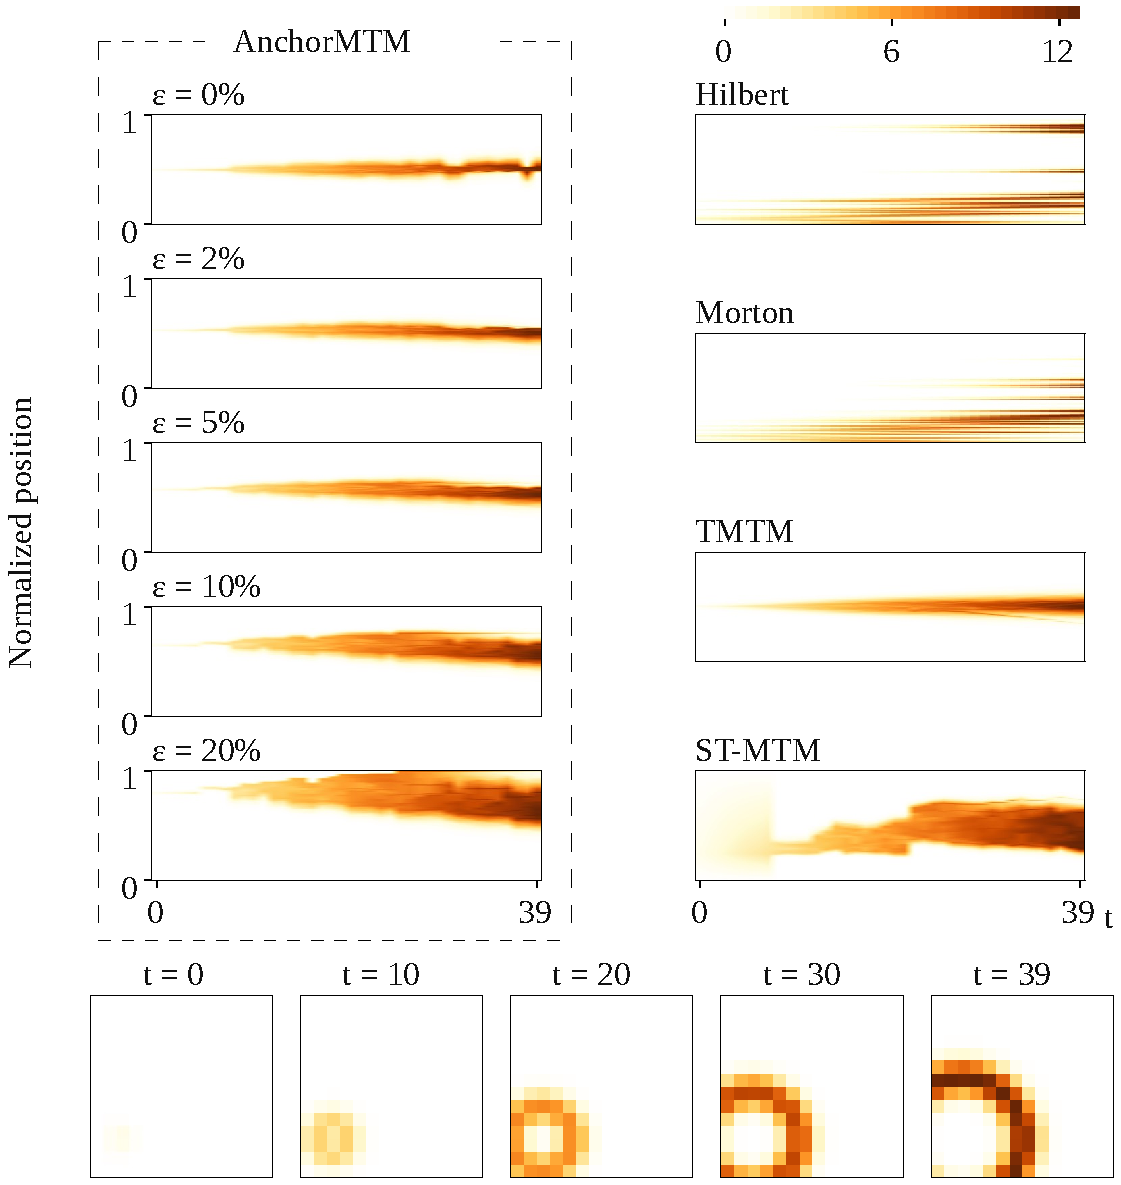
\includegraphics[width=\columnwidth]{figures/anchor_ring_result.pdf}
\caption{Ring: joint spatial guidance and merge allowances 0, 2, 5, 10 and 20\%, with same-input TMTM/ST-MTM maps, supplied curve panels and five source snapshots. All computed maps retain 40 frames and 196 positions.}
\label{fig:ring-result}
\end{figure}
\paragraph{Ring.} Figure~\ref{fig:ring-result} varies guidance jointly with budget: $q_{layout}=(1-\alpha)q_{mid}+\alpha q_{physical}$, with $\alpha=\varepsilon/20\%$ and a fixed $-128.7^\circ$ physical direction. Increasing guidance moves the ring toward its projected positions; the snapshots connect this change to expansion and strengthening.

\begin{figure}[!tb]
\centering
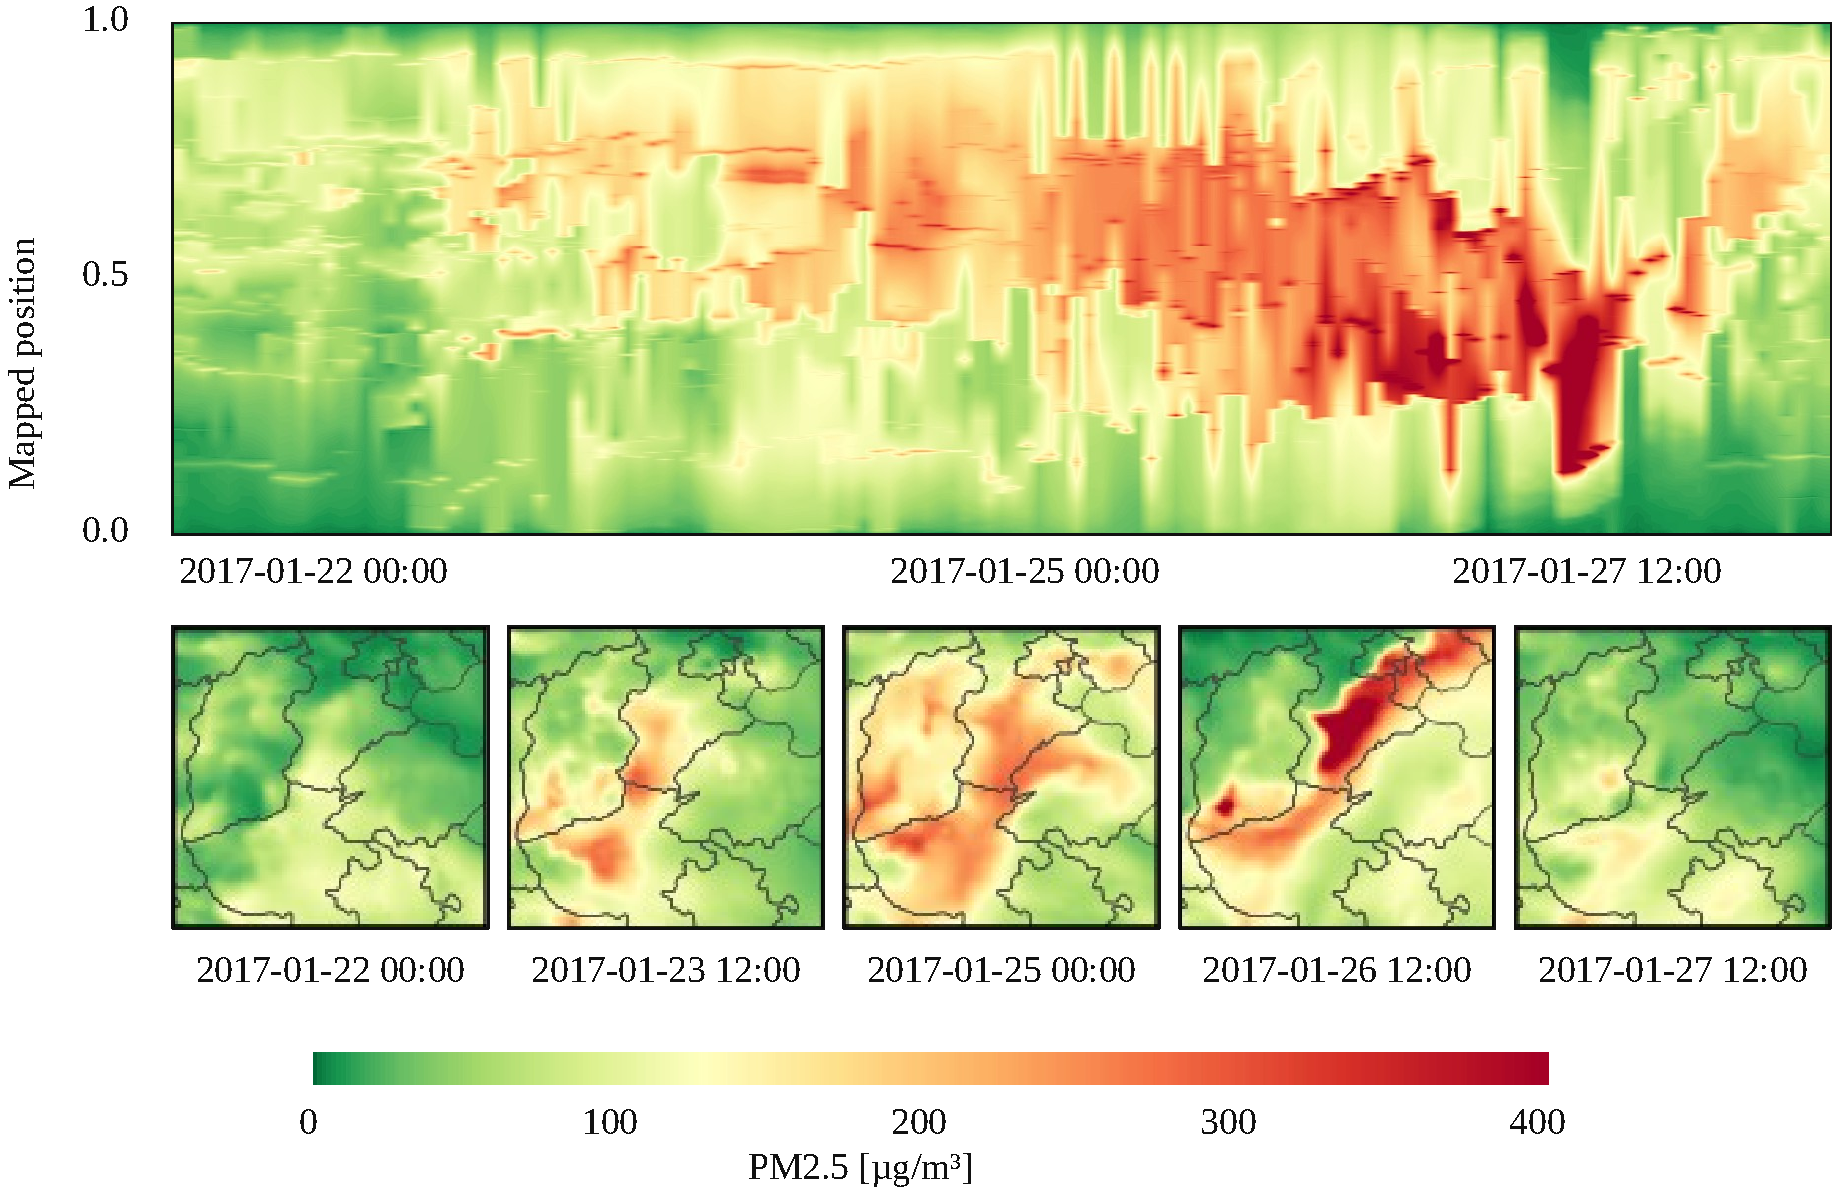
\includegraphics[width=\columnwidth]{figures/PM25_single_column.pdf}
\caption{Hourly PM2.5, January 22 00:00--27 12:00, 2017 (Beijing time): the 5\% map and five source snapshots. All 133 hourly samples are retained; concentrations above 400 $\mu$g/m$^3$ saturate.}
\label{fig:pm25-hourly}
\end{figure}
\paragraph{PM2.5.} Figure~\ref{fig:pm25-hourly} places a 133-hour event within the complete January sequence. Join trees of negated concentration represent high-concentration features, and the display restores positive concentration. The 5\% mode attains 4.998\% maximum merge error across all 744 hours. Snapshots provide the geographic context for the matched peak visible in the temporal map.

\subsection{Implementation and Runtime}
\paragraph{Verification pipeline.} The supplied code rebuilds the controlled-tree, feature-position and budget-distribution figures from labelled layouts and raster columns: 43 controlled overlaps, 364 controlled budgets, 9,168 planar frame--budget observations and 1,515 volumetric columns. For each volume column it reconstructs adjacent barriers from the original scalar raster, accumulates pairwise maxima and compares the complete fixed-label matrix with the source tree. It also verifies support IDs, interval order, canvas capacity, gaps and anchor slack. Every chart mark is then generated from the resulting CSV records. The five-sequence audit separately recomputes the point/width certificates and the baseline inversion errors in Table~\ref{tab:real-bounds}. These two checks link the rendered spatial-error distributions to the theoretical quantities used during ordering. Planar optimization takes 0.15--3.32\,s on the four benchmark inputs and 199.97\,s for the uncached PM2.5 Balanced run on Apple M4; full pipeline times and configurations appear in the supplement.

\paragraph{Configuration and runtime.} Tables~\ref{tab:anchor-parameters-final} and~\ref{tab:volume-parameters} give the fixed settings used by the quantitative comparisons. Only the merge allowance changes between each Exact--Balanced pair. The table runtimes measure one uncached run on Apple M4; optimization includes order search and anchor placement, while the total includes tree extraction, matching, filling and checks.
\begin{table}[!tb]
\centering
\caption{Planar parameter settings and runtime (seconds).}
\label{tab:anchor-parameters-final}
\footnotesize
\setlength{\tabcolsep}{2pt}
\renewcommand{\arraystretch}{0.95}
\begin{tabular}{@{}lccccc@{}}
\toprule
Parameter & Gaussian & Ring & Wildfires & Storms & PM2.5 \\
\midrule
$\varepsilon$ & 1\% & 1\% & 5\% & 10\% & 5\% \\
$N_r$ & 4096 & 196 & 4096 & 4096 & 4096 \\
$s_w$ & 0.00581 & 0.00328 & 0.00053 & 0.01170 & 0.00073 \\
$t_{opt}$ & 0.156 & 0.150 & 3.324 & 2.600 & 199.975 \\
$t_{total}$ & 1.340 & 0.486 & 4.424 & 63.447 & 231.177 \\
\bottomrule
\end{tabular}
\vspace{2pt}
\begin{minipage}{0.94\columnwidth}\footnotesize Weights $(4,1,0.5,0.1)$ and $\rho=0.5$ are fixed. $s_w$ is width per support measure; $N_r$ is raster length. PM2.5 uses $p=5\%$ of per-frame range and a fixed 5\% Balanced budget, without validation-set selection; both times are remeasured without a tree cache under the same pipeline scope. Times are one run on Apple M4: optimization and full pipeline, respectively.\end{minipage}
\end{table}

\begin{table}[!tb]
\centering
\caption{Volumetric datasets and Balanced-mode parameter settings.}
\label{tab:volume-parameters}
\footnotesize
\setlength{\tabcolsep}{2pt}
\renewcommand{\arraystretch}{0.95}
\begin{tabular}{@{}lcc@{}}
\toprule
Parameter & Cylinder & Tangaroa \\
\midrule
Frames & 102 & 201 \\
Grid & $135\times64\times48$ & $300\times180\times120$ \\
Scalar & $Q$-criterion & Speed $\|\mathbf{v}\|$ \\
Persistence & 2\% per-frame range & 0.2 absolute \\
Reference & $+x$ & $+x$ \\
$\varepsilon$ & 1\% & 33.33\% \\
$N_r$ & 32768 & 131072 \\
$s_w$ & $2.70668\times10^{-5}$ & 0.40953 \\
Weights & $(0.1,16,0,0.1)$ & $(0,64,0,0)$ \\
$\rho$ & 1 & 1 \\
Gap$/L_{world}$ & $1/300$ & $1/960$ \\
Extra$/L_{world}$ & 0.1 & 0.1 \\
\bottomrule
\end{tabular}
\vspace{2pt}
\begin{minipage}{0.94\columnwidth}\footnotesize Weights are reference, geometry, temporal and eccentricity. $s_w$ is width per support measure (Cylinder voxel counts; Tangaroa physical volume); $N_r$ is raster length, distinct from the physical canvas extent $L_{world}$. Exact uses zero allowance with the same other parameters as its Balanced counterpart.\end{minipage}
\end{table}

\Needspace{7\baselineskip}
